\section{Identificação do Modelo do Sistema}

O objetivo desta seção é determinar um modelo matemático linear que represente a dinâmica do sistema de levitação magnética em torno de um ponto de operação. A abordagem utilizada baseia-se na metodologia de identificação no domínio da frequência proposta por Kawakami et al.(2003).

\subsection{Modelo Teórico Linearizado}

A força eletromagnética $F_M$ exercida pelo solenoide sobre a esfera metálica é intrinsecamente não-linear, sendo proporcional ao quadrado da corrente $i$ e inversamente proporcional ao quadrado da distância $x$ entre eles, conforme a Equação \ref{eq:forca_mag}.
\begin{equation}
    F_{M} = k \frac{i^{2}}{x^{2}}
    \label{eq:forca_mag}
\end{equation}
onde $k$ é um coeficiente de conversão eletromecânica. A dinâmica completa do sistema é descrita por uma equação diferencial não-linear. Para fins de projeto de controle, é conveniente linearizar o sistema em torno de um ponto de equilíbrio.

Seguindo o trabalho de Kawakami, o modelo linearizado que relaciona a variação da tensão de controle na entrada, $u(s)$, com a variação da tensão do sensor na saída, $y(s)$, pode ser representado pela seguinte função de transferência: 
\begin{equation}
    G(s) = \frac{Y(s)}{U(s)} = -\frac{A}{s^2 - \eta}
    \label{eq:tf_kawakami}
\end{equation}
Neste modelo, $A$ é um ganho positivo e $\eta$ é um parâmetro relacionado à gravidade e à posição de equilíbrio da esfera ($ \eta = 2g/H_0 $). A presença de um polo em malha aberta em $s = +\sqrt{\eta}$ confirma a instabilidade inerente do sistema. O objetivo da identificação é, portanto, estimar os valores de $A$ e $\eta$ a partir de dados experimentais.

\subsection{Metodologia de Identificação}

A estimação dos parâmetros foi realizada no domínio da frequência. A resposta em frequência do modelo da Equação \ref{eq:tf_kawakami} é obtida substituindo $s = j\omega$:
\begin{equation}
    G(j\omega) = \frac{A}{\omega^2 + \eta}
    \label{eq:tf_jw}
\end{equation}
Note que $G(j\omega)$ é um valor puramente real, o que significa que a fase do sistema é de $0^\circ$ ou $180^\circ$, dependendo do sinal do ganho. O módulo (ganho linear) da resposta em frequência é, portanto, $|G(j\omega)|$. Manipulando a Equação \ref{eq:tf_jw}, podemos escrever uma relação linear para os parâmetros $A$ e $\eta$: 
\begin{equation}
    A - \eta \cdot \text{Gain}(\omega_i) = \omega_i^2 \cdot \text{Gain}(\omega_i)
    \label{eq:mq_linear}
\end{equation}
onde $\text{Gain}(\omega_i)$ é o ganho linear medido experimentalmente na frequência $\omega_i$. Coletando medições para um conjunto de $N$ frequências distintas, monta-se um sistema de equações lineares na forma matricial $P\theta = Q$, onde $\theta = [\eta, A]^T$. A solução de mínimos quadrados que minimiza o erro é dada por:
\begin{equation}
    \hat{\theta} = (P^T P)^{-1} P^T Q
\end{equation}

\subsection{Procedimento Experimental e Análise de Dados}

Para a coleta de dados, o sistema foi excitado com um sinal do chirp, abrangendo a faixa de frequências de interesse. Os sinais de tensão de entrada (controle) e de saída (sensor de posição) foram registrados e correspondem ao ponto de operação de -1V.

Utilizando o MATLAB, a resposta em frequência do sistema foi calculada através da Fast Fourier Transform (FFT) dos sinais de saída e entrada ($H(j\omega) = \text{FFT}(y(t)) / \text{FFT}(u(t))$). O Diagrama de Bode resultante, exibindo a magnitude e a fase da resposta em frequência experimental, é apresentado na Figura \ref{fig:bode}.

\begin{figure}[ht!]
    \centering
    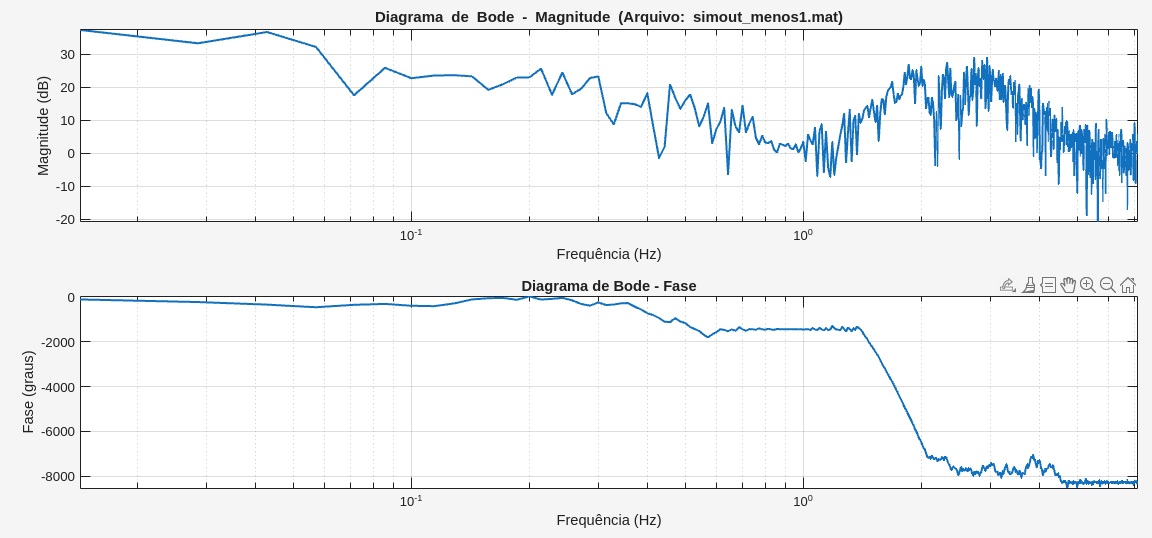
\includegraphics[width=0.5\textwidth]{bode_plot.png} % Use o nome do seu arquivo de imagem
    \caption{Diagrama de Bode experimental obtido a partir dos dados do ponto de operação -1V.}
    \label{fig:bode}
\end{figure}

\subsection{Resultados e Estimação dos Parâmetros}

A partir do gráfico de magnitude do Diagrama de Bode, os ganhos lineares foram extraídos para um conjunto de frequências discretas, conforme listado na Tabela \ref{tab:ganhos}.

\begin{table}[ht!]
    \centering
    \caption{Ganhos lineares extraídos da resposta em frequência experimental.}
    \label{tab:ganhos}
    \begin{tabular}{cc}
        \toprule
        \textbf{Frequência (Hz)} & \textbf{Ganho Linear} \\
        \midrule
        1.0                      & 1.4872                \\
        2.0                      & 20.4245               \\
        3.0                      & 13.8815               \\
        4.0                      & 5.4749                \\
        5.0                      & 0.2491                \\
        6.0                      & 1.4917                \\
        7.0                      & 2.8305                \\
        8.0                      & 1.9371                \\
        9.0                      & 1.9371                \\
        10.0                     & 1.9371                \\
        \bottomrule
    \end{tabular}
\end{table}

Aplicando o método dos mínimos quadrados com os dados da Tabela \ref{tab:ganhos}, obteve-se a seguinte estimativa para os parâmetros do modelo:
\begin{itemize}
    \item $\hat{\eta} = -27.2265$
    \item $\hat{A} = 3684.5816$
\end{itemize}
O valor estimado para $\eta$ resultou negativo. Fisicamente, um $\eta$ negativo implicaria em um sistema de malha aberta estável ($s^2 - \eta = s^2 + |\eta|$), o que contradiz a natureza instável do levitador magnético. Esse resultado pode ser atribuído a ruídos na medição ou a não-linearidades do sistema. Para garantir a coerência física do modelo, adotou-se o valor absoluto de $\eta$, ou seja, $\eta_{modelo} = |\hat{\eta}| = 27.2265$.

Com os parâmetros ajustados, a função de transferência estimada para o ponto de operação de -1V é:
\begin{equation}
    G(s) = -\frac{3684.58}{s^2 - 27.23}
    \label{eq:tf_final}
\end{equation}

\subsection{Validação do Modelo}

Para validar a precisão do modelo identificado, a resposta em frequência teórica (Equação \ref{eq:tf_jw}) foi plotada utilizando os parâmetros $\eta_{modelo}$ e $\hat{A}$. A Figura \ref{fig:validacao} compara esta curva teórica com os pontos de ganho obtidos experimentalmente.

\begin{figure}[ht!]
    \centering
    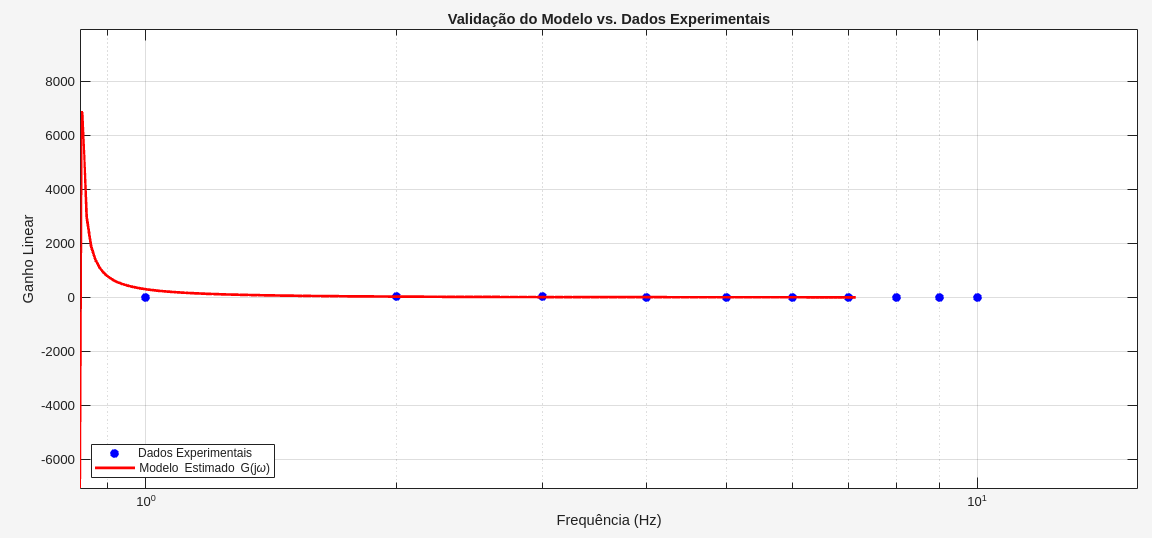
\includegraphics[width=0.5\textwidth]{modelovsreal.png} % Use o nome do seu arquivo de imagem
    \caption{Comparação entre os ganhos experimentais (pontos em azul) e a resposta em frequência do modelo estimado (curva em vermelho).}
    \label{fig:validacao}
\end{figure}

Observa-se uma boa aderência entre o modelo estimado e os dados experimentais, especialmente nas frequências mais baixas, que são mais dominantes na dinâmica do sistema. A discrepância em frequências mais altas pode ser atribuída a ruídos e dinâmicas não modeladas. A validação visual confirma que o modelo obtido é uma representação adequada do sistema para a finalidade de projeto de controladores.

\section{Projeto do Controlador e Simulação}

Com a função de transferência da planta $G(s)$ identificada na seção anterior, o próximo passo é projetar um controlador $C(s)$ que estabilize o sistema em malha fechada. Para esta tarefa, foi utilizada a ferramenta interativa SISOTOOL do MATLAB.

\subsection{Estratégia de Controle e Projeto no SISOTOOL}

A planta identificada, dada pela Equação \ref{eq:tf_final}, possui um polo instável no semiplano direito ($s = \sqrt{27.23} \approx +5.22$), tornando o sistema de malha aberta instável. A estratégia de controle deve, primeiramente, alocar todos os polos de malha fechada no semiplano esquerdo.

Para alcançar a estabilização, foi projetado um controlador com a seguinte estrutura:
\begin{itemize}
    \item \textbf{Dois zeros reais:} Zeros em $s = -1$ e $s = -2.8$ foram adicionados. No Lugar das Raízes, a função desses zeros é "puxar" o ramo do lugar geométrico que se inicia no polo instável para o semiplano esquerdo, forçando a estabilização do sistema.
    \item \textbf{Um integrador:} Um polo na origem ($s=0$) foi incluído para garantir que o sistema em malha fechada tenha erro nulo em regime permanente para uma entrada do tipo degrau, uma característica desejável para sistemas de posicionamento.
    \item \textbf{Um polo distante:} Um polo em $s = -500$ foi adicionado para tornar o controlador estritamente próprio. Isso limita o ganho em altas frequências, o que reduz a sensibilidade do sistema a ruídos e torna o controlador fisicamente mais realizável.
\end{itemize}

Após a inserção desses polos e zeros, o ganho do controlador foi ajustado interativamente no SISOTOOL para posicionar os polos de malha fechada em uma região que fornecesse uma resposta transitória adequada.

\subsection{Controlador Final Obtido}

A função de transferência resultante é dada pela Equação \ref{eq:controlador}.

\begin{equation}
    C(s) = -54.918 \frac{(s+2.8)(s+1)}{s(s+500)}
    \label{eq:controlador}
\end{equation}

O sinal negativo do ganho é necessário para garantir que a realimentação do sistema seja negativa, uma vez que a planta $G(s)$ possui um ganho estático negativo.


\subsubsection{Lugar das Raízes}

O Lugar das Raízes da malha aberta ($L(s) = C(s)G(s)$) é apresentado na Figura \ref{fig:root_locus}. O gráfico confirma a eficácia da estratégia de controle: os zeros em -1 e -2.8 atraem o polo instável da planta para o semiplano esquerdo. Os quadrados roxos indicam a posição final dos polos de malha fechada para o ganho escolhido, todos localizados no semiplano esquerdo, o que garante a estabilidade do sistema.

\begin{figure}[ht!]
    \centering
    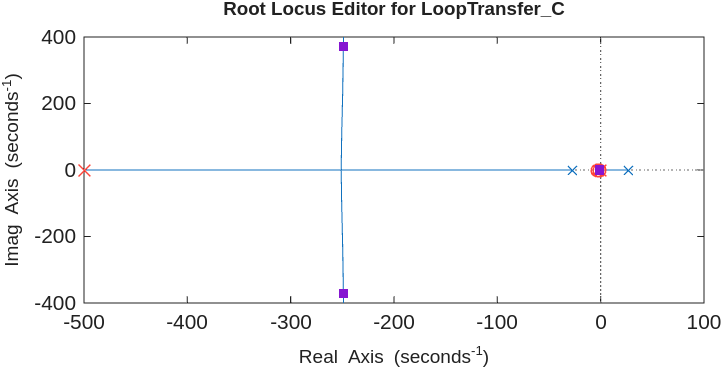
\includegraphics[width=0.5\textwidth]{root_locus.png}
    \caption{Lugar das Raízes para o sistema compensado. Todos os polos de malha fechada (quadrados roxos) estão no semiplano esquerdo.}
    \label{fig:root_locus}
\end{figure}
\newpage

\subsubsection{Análise no Domínio da Frequência}

O Diagrama de Bode da malha aberta é exibido na Figura \ref{fig:bode_loop}. O sistema apresenta uma \textbf{Margem de Fase de 55.6 graus}, um valor robusto que indica boa tolerância a atrasos no sistema.

\begin{figure}[ht!]
    \centering
    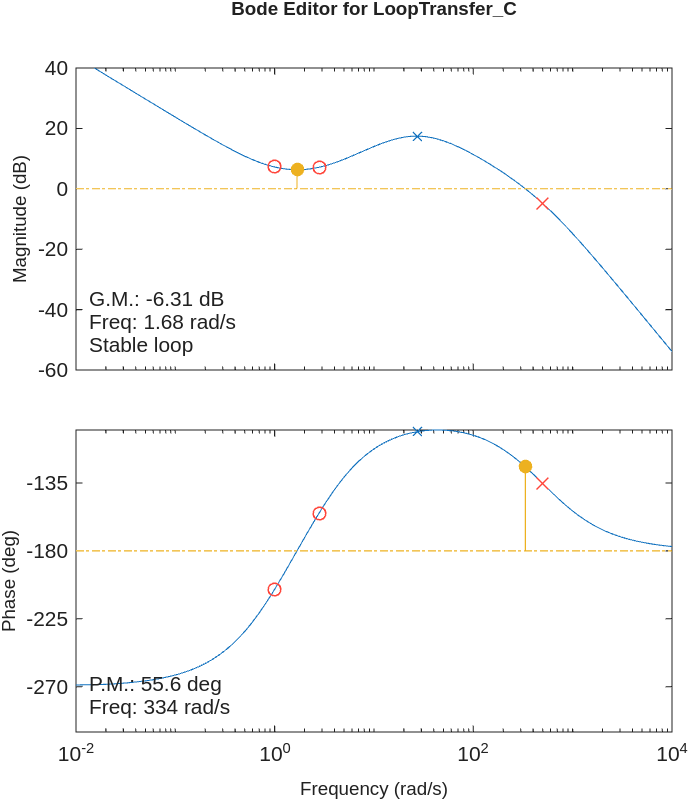
\includegraphics[width=0.5\textwidth]{bode.png}
    \caption{Diagrama de Bode do sistema em malha aberta ($L(s)=C(s)G(s)$).}
    \label{fig:bode_loop}
\end{figure}

Para uma análise de estabilidade definitiva, recorre-se ao Critério de Nyquist, mostrado na Figura \ref{fig:nyquist}. A planta $G(s)$ possui um polo no semiplano direito (P=1). Para que o sistema em malha fechada seja estável, o diagrama de Nyquist de $L(s)$ deve circular o ponto crítico (-1, 0) uma vez no sentido anti-horário (N=-1). Como Z = P + N = 1 + (-1) = 0, a ausência de polos de malha fechada no semiplano direito é confirmada, e a estabilidade do sistema é garantida.

\begin{figure}[ht!]
    \centering
    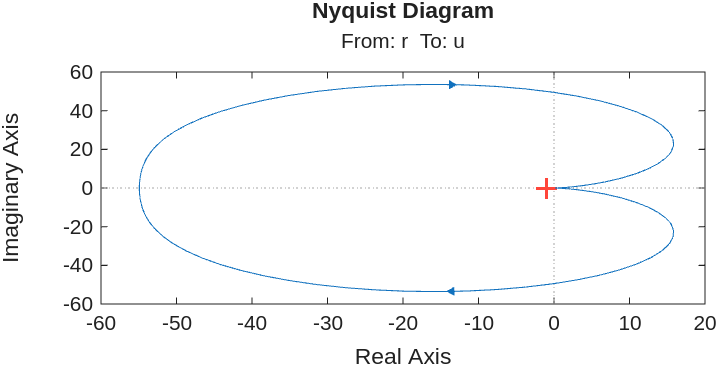
\includegraphics[width=0.5\textwidth]{nyquist.png}
    \caption{Diagrama de Nyquist confirmando a estabilidade do sistema (um enlace anti-horário em torno de -1).}
    \label{fig:nyquist}
\end{figure}
\newpage
\subsubsection{Resposta ao Degrau}

A Figura \ref{fig:step_response} mostra a resposta ao degrau para o sinal de controle (de referência 'r' para o atuador 'u'). A resposta é rápida, estabilizando-se em aproximadamente 0.015 segundos. O sobressinal observado no sinal de controle é uma consequência do esforço necessário para estabilizar rapidamente a planta inerentemente instável.

\begin{figure}[ht!]
    \centering
    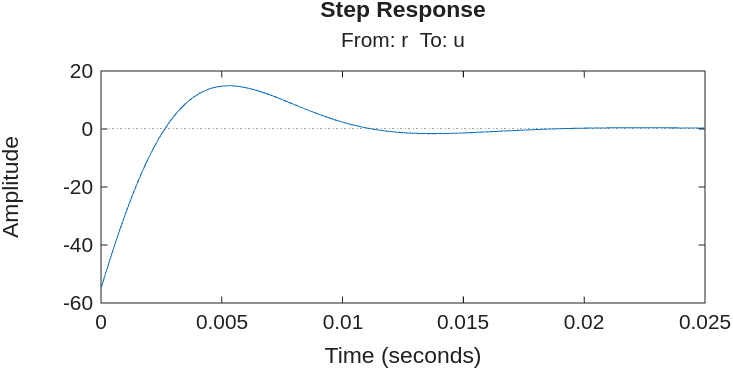
\includegraphics[width=0.5\textwidth]{step_resp.png}
    \caption{Resposta do sinal de controle ($u$) a uma entrada de referência em degrau ($r$).}
    \label{fig:step_response}
\end{figure}

Em conjunto, as análises demonstram que o controlador projetado estabiliza a planta de levitação magnética, também proporcionando um sistema em malha fechada com boa robustez e uma resposta rápida.

